\subsection{环的根}

定义 2. —— 环 A 的雅各布森根（或简称根），记作 \(\Re(\mathrm{A})\)，是 A-模 \(A_{s}\) 的根，即 A 的极大左理想之交。

滥用语言，若我们有 \(\Re(A)=0\)，则称环 A 是无根的。

命题 4. —— 环 A 是半单的，当且仅当它是左阿廷的且无根的。

这由把命题 3, b) 应用于 A-模 \(\mathrm{A}_s\) 得出。

例. —— 1) 若 A 是一个局部环，则它有唯一的极大左理想 r，由 A 的不可逆元素组成（VIII, 第 25 页，命题 1）；于是 r 是 A 的根。特别地，体是无根的。

\pandocbounded{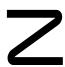
\includegraphics[keepaspectratio]{images/part001_b3b59696.jpg}}

\begin{enumerate}
\def\labelenumi{\arabic{enumi})}
\setcounter{enumi}{1}
\item
  设 K 是一个交换域，E 是形式幂级数代数 \(\mathrm{K}[[\mathrm{X}_{i}]]_{i\in\mathrm{I}}\)（变量 \(X_{i}\)、系数在 K 中）。由前一例以及 VIII, 第 26 页的例 4，E 的根由常数项为零的形式幂级数组成。注意环 E 是一个整环，且其根不归结为 0，尽管 E 是它的无根的分式域的一个子环。
\item
  设 A 是一个主理想整环，P 是由不可约元组成的一个代表系（VII, §1, No.~3, 第 3 页）。若 A 是一个体，则由例 1 它是无根的。若集 P 是无穷的，则 A 的诸极大理想 Ap 的交归结为 0，故 A 是无根的。但若 P 有限且非空，且我们令 \(x = \prod_{p \in P} p\)，则 A 的根等于 \(\cap_{p \in P} Ap = Ax\)（VII, §1, No.~2, 第 3 页，命题 4），因而不归结为 0。
\end{enumerate}

设 y 是 A 的一个非零元素；我们把它写成 \(y = up_{1}^{i_{1}} \cdots p_{r}^{i_{r}}\)，其中 u 在 A 中可逆，\(p_{1}, \ldots, p_{r}\) 是 P 中两两互异的元素，而 \(i_{1}, \ldots, i_{r}\) 是严格正的整数。环 A/Ay 的极大理想是诸理想 \(Ap_{1}/Ay, \ldots, Ap_{r}/Ay\)；因而环 A/Ay 的根是理想 \(Ap_{1} \cdots p_{r}/Ay\)。特别地，环 A/Ay 是无根的，当且仅当我们有 \(i_{1} = \cdots = i_{r} = 1\)；这时，我们称 y 是无重因子的。

命题 5. —— a) 环 A 的根是诸单 A-模的零化子之交；它也是半单 A-模的零化子中最小的一个。特别地，它是 A 的一个双边理想。若 A 不归结为 0，则 A 的根异于 A。

\begin{enumerate}
\def\labelenumi{\alph{enumi})}
\setcounter{enumi}{1}
\item
  设 \(\mathfrak{a}\) 是 A 的一个双边理想。我们有 \((\Re (\mathrm{A}) + \mathfrak{a}) / \mathfrak{a} \subset \Re (\mathrm{A} / \mathfrak{a})\)。若 \(\mathfrak{a}\) 包含于 \(\Re (\mathrm{A})\)，则我们有 \(\Re (\mathrm{A} / \mathfrak{a}) = \Re (\mathrm{A}) / \mathfrak{a}\)。
\item
  环 A/R(A) 是无根的；反之，A 的每个使 A/a 为无根的双边理想 a 都包含 R(A)。
\item
  A 的根包含于 A 的诸极大双边理想之交。
\end{enumerate}

设 \(x \in \mathrm{A}\)。说 \(x\) 属于每个单 A-模的零化子，等价于说 \(x\) 属于每个单 A-模的每个元素的零化子，换句话说（VIII, 第 46 页，命题 1），等价于属于 A 的每个极大左理想。

设 M 是一个半单 A-模。它的零化子是 M 的诸单子模的零化子之交，故它包含 \(\Re(\mathrm{A})\)。此外，若 S 是单 A-模的类所成的集（VIII, 第 51 页），则直和 \(\oplus_{\lambda\in\mathcal{S}}\lambda\) 是一个零化子为 \(\Re(\mathrm{A})\) 的半单 A-模。设 A 不归结为 0；则关系 \(\Re(\mathrm{A})\neq\mathrm{A}\) 由把 VIII, 第 153 页的命题 2, a) 应用于 A-模 \(A_{s}\) 而得。我们证明了 a)。

设 \(\mathfrak{a}\) 是 A 的一个双边理想。A/ \(\mathfrak{a}\) 的极大左理想是形如 \(\mathfrak{m}/\mathfrak{a}\) 的理想，其中 \(\mathfrak{m}\) 是 A 的包含 \(\mathfrak{a}\) 的一个极大左理想。因而环 A/ \(\mathfrak{a}\) 的根等于 A-模 \(A_s/\mathfrak{a}\) 的根。于是断言 b) 与 c) 由 VIII, 第 152 页的推论 1 得出。

设 \(\mathfrak{a}\) 是 A 的一个极大双边理想。在环 A/ \(\mathfrak{a}\) 中，仅有的双边理想是 0 与 A/ \(\mathfrak{a}\)。由于环 A/ \(\mathfrak{a}\) 不归结为 0，它的根不等于 A/ \(\mathfrak{a}\)。因而环 A/ \(\mathfrak{a}\) 是无根的，且由 c) 我们有 \(\Re(A) \subset \mathfrak{a}\)。这就证明了 d)。

我们称 A 的一个左（或右）理想是诣零理想，如果它由幂零元素组成。我们称 A 的一个双边理想 \(\mathfrak{a}\) 是幂零的，如果存在一个整数 \(n \geqslant 1\) 使得 \(\mathfrak{a}^n = 0\)，即（I, §8, No.~9, 第 107 页）使得我们有 \(x_1 \cdots x_n = 0\)，只要 \((x_1, \ldots, x_n)\) 是 \(\mathfrak{a}\) 中元素的一个序列。每个幂零双边理想都是诣零理想，但可能存在不包含于任何幂零双边理想之中的诣零理想（VIII, 第 167 页，习题 9）。

定理 1（雅各布森）. —— 环 A 的根由这样的元素 \(x \in \mathbf{A}\) 组成：\(1 + ax\) 对每个 \(a \in \mathbf{A}\) 都是左可逆的（I, §2, No.~3, 第 15 页）。它也是最大的双边理想 \(\mathfrak{a}\)：\(1 + x\) 对每个 \(x \in \mathfrak{a}\) 都可逆。\(\mathbf{A}\) 的根包含 \(\mathbf{A}\) 的每个左诣零理想。

元素 1 生成 A-模 \(A_{s}\)，且 \(1 + ax\) 左可逆当且仅当它生成 A-模 \(A_{s}\)。因而定理 1 的第一个断言是命题 2 的推论（VIII, 第 153 页）的一个特例。

设 \(x \in \Re(\mathrm{A})\)。由上述，\(1 + x\) 左可逆；设 \(y\) 是 \(\mathrm{A}\) 中使 \(y(1 + x) = 1\) 的一个元素。于是我们有 \(1 - y = yx\)，故 \(1 - y\) 属于 \(\Re(\mathrm{A})\)；因而 \(y\) 左可逆。由于 \(y\) 也右可逆，它可逆（I, §2, No.~3, 第 16 页，命题 3），而它的右逆 \(1 + x\) 也可逆。

设 a 是 A 的一个左理想，使得 \(1 + x\) 对每个 \(x \in a\) 都可逆。例如当 a 是诣零理想时即属此情形，因为关系 \(x^{n} = 0\) 蕴含 \(1 - x + \cdots + (-x)^{n-1}\) 是 \(1 + x\) 的逆。设 \(x \in a\)。对每个 \(a \in A\)，我们有 \(ax \in a\)，故 \(1 + ax\) 可逆；因而我们有 \(x \in \Re(A)\)。于是 a 包含于 \(\Re(A)\)。

推论 1. —— A 的根等于反环 A° 的根，即 A 的极大右理想之交。

对每个 \(x \in \Re(A)\)，\(1 + x\) 在环 A 中可逆，因而在环 \(A^{\circ}\) 中可逆。由于 \(\Re(A)\) 是 \(A^{\circ}\) 的一个双边理想，我们有 \(\Re(A) \subset \Re(A^{\circ})\)。交换 A 与 \(A^{\circ}\) 的角色即得等式。

推论 2. —— A 的一个元素可逆，当且仅当它在环 A/ \(\Re(A)\) 中的典范像可逆。

该条件显然是必要的。我们来证明它是充分的。设 x 是 A 的一个元素，它在环 \(\mathrm{A}/\Re(\mathrm{A})\) 中的典范像可逆。则存在 A 的一个元素 y，使得 xy 属于 \(1 + \Re(\mathrm{A})\)。由定理 1，xy 可逆；因而 x 右可逆。x 左可逆的证明是类似的。

推论 3. —— 一族环 \((\mathrm{A}_{i})_{i\in\mathrm{I}}\) 的乘积的根是诸 \(\mathfrak{R}(\mathrm{A}_{i})\) 的乘积。

设 \(x = (x_{i})_{i\in \mathrm{I}}\) 是 \(\prod_{i\in \mathrm{I}}\mathrm{A}_{i}\) 的一个元素。对每个元素 \(a = (a_{i})_{i\in \mathrm{I}}\)（\(\prod_{i\in \mathrm{I}}\mathrm{A}_{i}\) 的），元素 \(1 + ax\) 左可逆当且仅当 \(1 + a_{i}x_{i}\) 在 \(\mathrm{A}_i\) 中左可逆（对每个 \(i\in \mathrm{I}\)）。由此即得推论 3。

推论 4. —— 环 A 是局部的，当且仅当环 A/ \(\Re(A)\) 是一个体。若属此情形，则 \(\Re(A)\) 是 A 的不可逆元素所成的集。

用 r 表示 A 的不可逆元素所成的集。若环 A 是局部的，则它的根等于 r（VIII, 第 154 页，例 1），且环 A/r 是一个体（VIII, 第 26 页）。反之，设环 A/R(A) 是一个体。由推论 2，我们有 \(\mathfrak{r} = \Re(\mathrm{A})\)，故 r 是 A 的一个双边理想。由此推得环 A 是局部的（VIII, 第 26 页，定义 1）。

例. —— 4) 设 K 是一个整环，I 是一个非空集，A 是多项式环 \(K[X_{i}]_{i\in I}\)。我们来证明环 A 是无根的。A 中仅有的可逆元素是 K 的可逆元素（IV, §1, No.~5, 第 9 页，推论 2）。设 \(f \in \Re(A)\)。选取一个元素 \(i \in I\)。则 \(1 + fX_{i}\) 可逆（定理 1），这蕴含 f = 0。

\pandocbounded{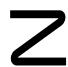
\includegraphics[keepaspectratio]{images/part001_fdd5464e.jpg}}

注意当 K 是一个交换域时，环 \(A = K[X_{i}]_{i \in I}\) 是 \(B = K[[X_{i}]]_{i \in I}\) 的一个子环，且我们有 \(\Re(A) = 0\) 与 \(A \cap \Re(B) \neq 0\)（参见 VIII, 第 154 页，例 2）。

\begin{enumerate}
\def\labelenumi{\arabic{enumi})}
\setcounter{enumi}{4}
\tightlist
\item
  设 \(\mathfrak{a}\) 是 A 的一个双边理想。A 上的 \(\mathfrak{a}\)-进拓扑是与 A 的环结构相容、且使诸理想 \(\mathfrak{a}^n\)（对 \(n \geqslant 1\)）构成 0 的一个基本邻域系的那个拓扑（《一般拓扑》，III, §6, No.~3, 第 275 页，例 3）。设环 A 对此拓扑是豪斯多夫的且完备的（《一般拓扑》，III, §6, No.~5, 第 276 页）；例如当理想 \(\mathfrak{a}\) 幂零时即属此情形。于是对每个 \(x \in \mathfrak{a}\)，级数 \(\sum_{n=0}^{\infty} (-x)^n\) 收敛。设 \(y\) 是它的和。我们有 \(y - 1 = \sum_{n=1}^{\infty} (-x)^n = -xy\)，因而 \((1 + x)y = 1\)。同样，我们有 \(y(1 + x) = 1\)，故 \(1 + x\) 可逆。由定理 1，由此推得理想 \(\mathfrak{a}\) 包含于 A 的根中。
\end{enumerate}

注. —— 1) 由定理 1，环 A 的每个左诣零理想都包含于它的根中。设 x 是 A 的一个幂零的中心元素；则 Ax 是 A 的一个诣零理想，故 x 属于 A 的根。然而，可能存在 A 的非零幂零元素，而 A 却是无根的。例如，对每个整数 \(n \geqslant 2\)，体 K 上的矩阵环 \(\mathbf{M}_{n}(\mathrm{K})\) 是单的，因而是无根的（VIII, 第 154 页，命题 4），而它含有幂零元素，例如矩阵单位 \(E_{ij}\)（\(i \neq j\)）。

\pandocbounded{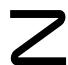
\includegraphics[keepaspectratio]{images/part001_653588be.jpg}}

\begin{enumerate}
\def\labelenumi{\arabic{enumi})}
\setcounter{enumi}{1}
\tightlist
\item
  设 A 是一个交换环。A 的幂零元素 \(a\) 所成的集是 A 的一个理想 \(\mathfrak{N}(\mathrm{A})\)，称为 A 的幂零根；它是 A 的诸素理想之交（V, §15, No.~1, 第 118 页，命题 2）。我们有 \(\mathfrak{N}(A) \subset \mathfrak{R}(A)\)；*当 A 是一个阿廷环（VIII, 第 173 页，推论 2）或是交换域上的一个有限生成交换代数（《交换代数》，V, §3, n°4, 定理 3）时，我们有等式*。我们当然可能有 \(\mathfrak{N}(A) \neq \mathfrak{R}(A)\)。当 A 是环 K{[}{[}X{]}{]}（其中 K 是一个交换域）时即属此情形：这时我们有 \(\mathfrak{N}(A) = 0\) 与 \(\mathfrak{R}(A) = AX\)（VIII, 第 154 页，例 2）。
\end{enumerate}

